\documentclass[12pt,a4paper]{article} 

\title{NeuroField Reference}
\date{\today}

\usepackage{listings}
\usepackage{hyperref}
\usepackage{graphicx}
\usepackage[top=2cm,bottom=2cm,left=1.3cm,right=1.3cm]{geometry}
\usepackage{multirow}
%\usepackage{lscape}

\pagestyle{plain}
\parindent=0.0cm
\parskip=0.5cm

%\textheight=25cm
%\textwidth=16.3cm
%\oddsidemargin=0.0cm
%\evensidemargin=0.0cm
%\marginparwidth=0.0cm
%\marginparsep=0.0cm
%\topmargin=0.0cm
%\headheight=0.0cm
%\headsep=0.0cm
\footskip=1.3cm

\lstset{
basicstyle=\small\small\ttfamily,
frame=single,	        % adds a frame around the code
breaklines=true,		% sets automatic line breaking
breakatwhitespace=tru,	% sets if automatic breaks should only happen at whitespace
}
\newcommand{\code}[1]{ 
\begin{lstlisting}
#1
\end{lstlisting}
}
\newcommand{\type}[1]{ {\small\small\tt #1} }

\begin{document}

\maketitle
\abstract{\type{NeuroField} is a computer program (accompanied with helper scripts) that solves the neural field model of Robinson et al. \type{NeuroField} allows generalization of the corticothalamic model by allowing users to specify an arbitrary number of populations and their coupling response, dendritic response, firing response and axonal propagation via a configuration file; all objects may have independent parameter values. Output is also determined by the configuration file. This document is a reference of \type{NeuroField} for both users and developers.}
\tableofcontents

\pagebreak
\section{Users guide}

This users guide covers the obtaining, setting up, configuring and launching of \type{NeuroField}.

\subsection{Obtaining and setting up NeuroField}
svn set up

\subsection{Directory layout}
Within the main directory, the user can find:

\begin{tabular}{l p{12cm}}
\type{*.h, *.cpp}& C++ source code.\\
\type{Configs/}& Stores configuration files for \type{NeuroField}.\\
\type{Documentation/}& \type{Documentation/doc.tex} is the latex file for generating this document. Running \type{make doc} produces this document in \type{pdf} format, and \type{make clean} removes all the files latex produced (including \type{doc.pdf} and excluding \type{doc.tex}).\\
\type{helper\_scripts/}& Stores helper scripts, including plotting routines and other post-processing of data procedures.\\
\type{NeuroField}& A launcher script that handles compilation and launching of \type{NeuroField}, capable of automating parameter sweeps and submitting jobs in \type{yossarian}. Not to be confused with the executable \type{Release/NeuroField}.\\
\type{Output/}& When using the launcher script to sweep over parameters, the launcher script produces this directory, which stores all output files \type{neurofield.*} in independent subdirectories.\\
\type{Release/}& All compiled files, including the object files and the \type{NeuroField} executable is stored here. This directory will be deleted by \type{make clean}, so user data should not be stored here.\\
\type{neurofield.*}& Output files of \type{NeuroField}.
\end{tabular}

\subsection{Using NeuroField via launcher script}

\begin{enumerate}

\item Edit Makefile: Identify the platform to run NeuroField, and comment/uncomment the appropriate \type{COMP} and \type{CP} directions. Generally, this step is not needed, but users are encouraged to check.

\item To execute with only one set of parameters, edit your configuration file in \type{./Configs}, then run
\begin{lstlisting}
./NeuroField Configs/config_file
\end{lstlisting}
For example,
\begin{lstlisting}
./NeuroField Configs/conf.emirs
\end{lstlisting}
The output will be stored in the current directory.\footnote{Tips for \type{vi} users: you can launch \type{NeuroField} in \type{vi} with \type{:!./NeuroField \% [optional params]} }

\item To ease parameter exploration, the launcher script is capable of doing parameter sweeps. The launcher script supports sweeping over an arbitrary number of objects, parameters and runs. For example, if the user wants to launch \type{NeuroField} 3 times, with parameters varying according to the following table,

\begin{tabular}{l l r r r}
Object(s)&Parameter&1\textsuperscript{st} run&2\textsuperscript{nd} run&3\textsuperscript{rd} run\\
\hline
\type{Propagator 1}, \type{Propagator 2}&\type{gamma}&10&20&30\\
\type{Coupling data 1}&\type{Nu}&1&2&3
\end{tabular}

simply list the above table entries into the argument list:
\begin{lstlisting}
./NeuroField Configs/conf.emirs 'Propagator 1' 'Propagator 2' gamma 10 20 30 'Coupling data 1' Nu 1 2 3
\end{lstlisting}

In terms of syntactic restriction, each row in the table can have an arbitary number of objects, but only one parameter; every row must have the same number of runs.

\item In case the script is executed on \type{yossarian}, the launcher script tries to find a file called \type{pbs}. If no such file is found, the user would be prompted for a job name, expected computational time and email to generate \type{pbs}. This file is then submitted to the PBS system.

\item To clean up the directory, delete or store your \type{neurofield.*} output files and the \type{Output/} directory and subdirectories. Then run
\begin{lstlisting}
make clean
\end{lstlisting}
to delete \type{./Release/} and the files latex produced in \type{Documentation/}.

\item This documentation can be generated by running 
\begin{lstlisting}
make doc
\end{lstlisting}
which produces \type{./Document\-ation.pdf}. \type{make clean} deletes the files (including \type{./Document\-ation.pdf}) created by latex.

\end{enumerate}

\subsection{Using NeuroField executable without launcher script}
\label{sec:exe}

It is possible to use the launcher script in virtually all cases, so that a user may skip this section. A notable exception is to restart a completed simulation with a \type{neurofield.dump} file. If a user wishes to use the \type{./Release/NeuroField} executable without the launcher script, then compile it by running
\begin{lstlisting}
make
\end{lstlisting}
The \type{NeuroField} executable and object files are produced in \type{./Release/}.

The \type{./Release/NeuroField} executable runs in one of two modes, initial run mode and restart mode.

(1) In inital run mode \type{NeuroField} takes input from an \type{neurofield.conf} file initializes the simulation and then takes specified number of integration steps writing out a \type{neurofield.output} file and a \type{neurofield.dump} file for restarting.  The input filename can be changed on the command line by using the switch \type{-i newinputfilename}. Similarly the name of the output filename which defaults to \type{neurofield.output} can be changed via the switch \type{-o newoutputfilename}. The dump file which defaults to \type{neurofiled.dump} can be changed via \type{-d newdumpfilename}.

(2) The code dumps sufficient data about parameter values to restart. In restart mode the simulation will continue where it left off. Restart mode is accessed by running the code with command \type{Neurofield restart} rather than the usual \type{Neurofield} command on the command line. In order to run the code in restart mode it is necessary to take the \type{neurofield.dump} file which was produced from the run which will be restarted to be renamed as the new \type{neurofield.conf} file. The new \type{neurofield.conf} file should also be changed to reflect the new number of timesteps etc.  Note:- A restarting \type{neurofield.conf} file has different content to an initial run \type{neurofield.conf} and can only be used in restart mode.

\subsection{Writing a configuration file}

\type{NeuroField} takes in a configuration file to build its population and their properties, as well as generate output. This section documents ways to write a configuration file.

All configuration files are stored in \type{./Configs}. Users can write their own config files by editting existing ones. Alternatively,
\begin{lstlisting}
./NeuroField write defaults
\end{lstlisting}
generates a default configuration file to the present working directory.

To write a configuration file, a user can follow these steps:
\begin{enumerate}
\item Obtain an existing config file, using the above options. This is less tedious (and less error prone) than writing a new one from scratch.
\item Determine your population model by drawing a schematic diagram. An example is shown in Fig.~\ref{fig:pop}.
\item Specify the global parameters and connectivity matrix (Sec.~\ref{sec:global}).
\item Specify all populations (Sec.~\ref{sec:pop}).
\item Specify all propagators (Sec.~\ref{sec:prop}).
\item Specify all coupling (Sec.~\ref{sec:couple}).
\item Specify all output requests (Sec.~\ref{sec:output}).
\end{enumerate}

\begin{figure}\begin{center}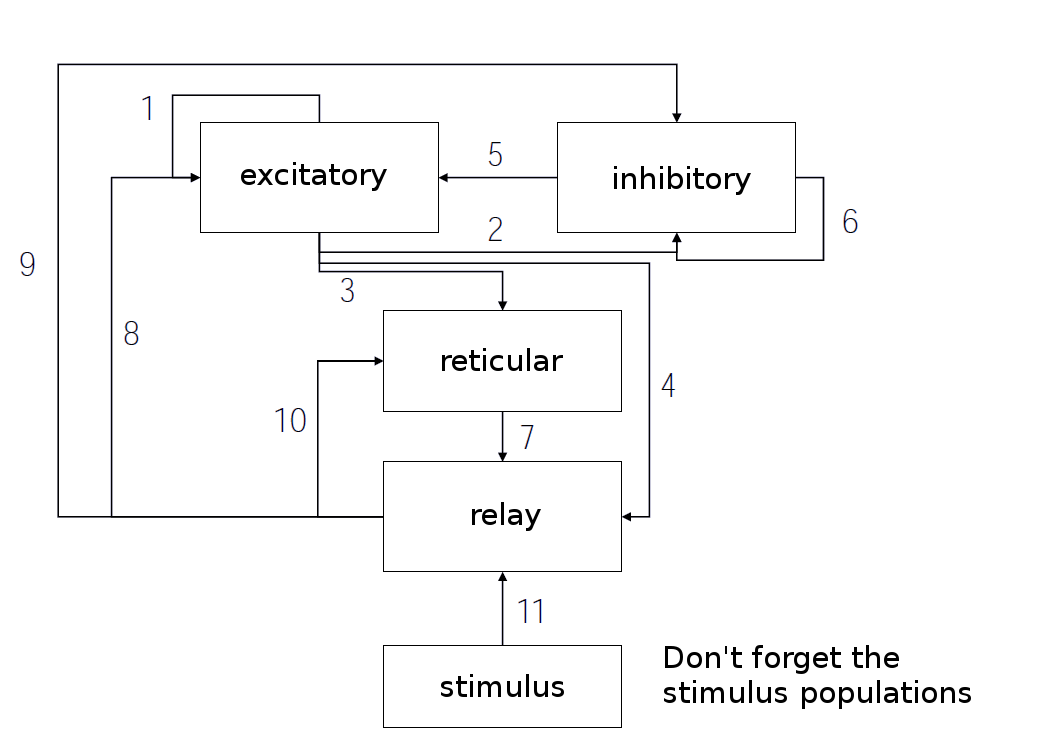
\includegraphics[scale=0.4]{pop.png}\caption{An example population model. Note all populations, including the stimulus population, are named, and all connections numbered for human referencing.}\label{fig:pop}\end{center}\end{figure}

The configuration file follows a logical structure: first the global simulation information, next the information for each populations given, then the propagation data, then the coupling data and finally the output data. Each component is described in detail below; each bullet point corresponds to a line of the input file.

\subsubsection{Global information}
\label{sec:global}
\begin{itemize}

\item The first line of the input file is skipped to allow the user to have a title
line
\item
\begin{lstlisting}
Nodes per population: 2500
\end{lstlisting}
This line contains the number of grid points in the spatial dimension per population of neurons. The code has been explicitly designed to have equal number of neurons per population.

Both spatial dimensions have periodic boundary conditions, so that populations have the topology of a torus.
\item
\begin{lstlisting}
Number of neural populations: 5
\end{lstlisting} This is the number of neural
populations and includes the number of stimulus modes. It is denoted
$n$ in this document.
\item
\begin{lstlisting}
Number of neural connections: 11
\end{lstlisting} This is the number of neural
populations which are connected together. By definition this number lies in the
range $n$ and $n^2$ where $n$ is the number of neural populations.
\item A blank line is inserted in the file at this point
\item
\begin{lstlisting}
Populations connections matrix 1 2 3 4 ....
\end{lstlisting} The code ignores this
line but it is useful to provide a way of lining up the data in the
connections matrix.
\item Now follows $n$ lines of connection matrix data. On each line the code looks for colon character followed by a number. There should be $n$ colons followed by a number on each line.
	
The row number corresponds to the population ID number of the TO population. The column number corresponds to the population ID number of the FROM population of the connection.

Zeros correspond to unconnected populations whilst nonzero number correspond to connected populations. For easy of use it is suggested that each connection be numbered in ascending order when reading down columns as in the default input file. This allows human crosschecking with later sections of the input file.
\item
\begin{lstlisting}
Number of integration steps: 100000 Skippoints: 49 Deltat: 0.0001
\end{lstlisting}
The parameters are: 
(1) the number of integration steps the code should step forward during the run, (2) An optional parameter of how many integration steps should be skipped before a time step should be outputted, and (3) the time increment for each time step.

\item
\begin{lstlisting}
Q delay depths: 420 :0 :0 :420 :0
\end{lstlisting} This line is no longer required 
and is ignored.

\item
\begin{lstlisting}
Propagator types 1: Waveeqn 2: Waveeqn 3: Waveeqn 4: Waveeqn 5: Mapping $
6: Mapping 7: Mapping 8: Waveeqn 9: Waveeqn 10: Mapping 11: Mapping $
\end{lstlisting}
These lines specifies the type of the $n$ propagator, each preceeded by an index number and a colon. The propagation data should appear in the same order as in the connection matrix when the connection matrix is read top to bottom and then left to right.

The following types of propagator are available: \type{Mapping}, \type{Waveeqn},\type{Waveeqnrect}, \type{Harmonic}, \type{Eqnset}, \type{Eqnsetrect}.
\item
\begin{lstlisting}
Coupling types 1: Modulate 2: Simple 3: Simple 4: Simple 5: Simple 6: Simple $ 
7: Simple 8: Simple 9: Simple 10: Simple 11: Simple $
\end{lstlisting}
These lines specifies the type of the $n$ couplings, each preceeded by an index number and a colon. The coupling data should appear in the same order as in the connection matrix when the connection matrix is read top to bottom and then left to right.

The following types of coupling are available: \type{Simple}, \type{Modcouple}, \type{STDP}, \type{Calcium}.
\item
\begin{lstlisting}
Lambda: 3e-4 tGlu: 5e-3
\end{lstlisting}
Parameters governing glutamate dynamics, which is currently useful only for \type{Calcium} type coupling. \type{Lambda} is the glutamate release concentration per presynaptic spike, in moles. \type{tGlu} is the decay timescale of glutamate in seconds.
\item A blank line finishes this section of the input file.
\end{itemize}

\subsubsection{Population data}
\label{sec:pop}
This section contains $n$ repeated population information sections.
Each population is presented in the same order as the connections matrix.
There are two types of neural populations: 1) ordinary populations
and 2) stimulus populations:
\begin{description}
\item[Ordinary populations]\ \\

	\begin{itemize}
	\item
	\begin{lstlisting}
Population 1 - Excitory neurons
	\end{lstlisting}
	The first line is ignored by the code but should be used for a text description of the population's name.
	\item
	\begin{lstlisting}
Initial Q: 8.87145
	\end{lstlisting}
	When the simulation starts an initial value for the firing rate $Q$ is required.
	\item
	\begin{lstlisting}
Firing Response Theta: 0.013 Sigma: 0.0038 Qmax: 250.0
	\end{lstlisting}
	These are the parameters of the population sigmoid firing response. Note the sigma value accepted by the code is in some Robinson papers it is known as $\tilde{\sigma}$. It is already scaled  by $\pi / \sqrt{3}$.

	An alternative syntax is
	\begin{lstlisting}
Firing Response Sigmoid: Theta: 0.013 Sigma: 0.0038 Qmax: 250.0
	\end{lstlisting}
	Alternatively, you can specify a linear firing response by using
	\begin{lstlisting}
Firing Response Linear: Gradient: 1 Intercept: 1
	\end{lstlisting}
	\item
	\begin{lstlisting}
Number of Dendritic responses: 3
	\end{lstlisting}
	The code uses this line purely for crosschecking purposes. It is equal to the number of populations whose connections terminate on the dendrites of the current population i.e. the number of non-zero elements in the column of the connection matrix of this population. We shall denote this number $m$.
	\item Now follow $m$ lines of dendritic response data. A complete dendritic response input line is given by
	\begin{lstlisting}
Dendritic Response from population 3 V initial: 0.0106457 alpha: 75.0 beta: 285.0
	\end{lstlisting}
	Each Dendritic response data line begins with an optional preamble which is ignored by the code. It is strongly suggested that for human readability this should be of the form {\tt \small Dendritic Response from population 3}.

	The following three parameters are the initial value of the subvoltage $V_{ab}$ and the parameters $\alpha_{ab}$ and $\beta_{ab}$ of the dendritic response differential equation. It should be noted the code has a separate dendritic response differential equation for each different population synapsing on the dendritic tree.
	
	The subvoltage $V_{ab}$ is the voltage in the dendrite due to incoming connections from population $b$. In some earlier papers all pulse densities were summed before a single differential equation described the total voltage in the dendritic tree. This code allows different dendritic responses for pulse densities arriving from different populations. If each dendritic response in a population has the same alpha and beta values the earlier case is effectively reproduced.
	
	If all coupling are \type{Simple}, and the initial $V_{ab}$ is given by the initial values of $\nu_{ab}$ and $\phi_{ab}$ via $V_{ab}= \nu_{ab} \phi_{ab}$, as in a steady state, then the dendritic response may be given as
	\begin{lstlisting}
Dendritic Response from population 3 V initial: Steady alpha: 75.0 beta: 285.0
	\end{lstlisting}
	\item A blank line finishes each population information section.
	\end{itemize}

\item[Stimulus populations]\ \\

The code identifies stimulus populations as populations which have no connections from other populations on their dendritic tree i.e., The column for that population contains no nonzero elements.  Each stimulus population information section is as follows.
\begin{itemize}
	\item \begin{lstlisting}
Population 5 - Stimulus neurons
	\end{lstlisting}
	The first line is ignored by the code but should be used for a text description of the population's name.
	\item
	\begin{lstlisting}
Initial Q: 8.87145
	\end{lstlisting}
	When the simulation starts an initial value for the firing rate $Q$ is required.
	\item The final line depends on the type of stimulus. Examples are:\\

	Pulse stimulus pattern:
	\begin{lstlisting}
Stimulus mode: 1 Time to start of stimulus: 0.002 Amplitude: 20 Pulse Duration: 0.02 Pulse repetition period: 0.005
	\end{lstlisting}

	White noise stimulus pattern (spatially uncorrelated), where Ranseed
is an optional parameter for the random number generator's initial seed defaulting to -98716872:
	\begin{lstlisting}
Stimulus mode: 2 Time to start of stimulus: 0.002 Ranseed:-98716872 Amplitude: 20
	\end{lstlisting}

	A ``special" stimulus pattern is the composite pattern, evoked by Stimulus mode 0. It takes in the time onset of an arbitrary number of arbitrary stimulus patterns, followed by the details of each stimulus pattern:
	\begin{lstlisting}
Stimulus mode: 0 Time to start of stimulus: 0 5 10 $
Stimulus mode: 7 Time to start of stimulus: 0.0000 Mean: 0
Stimulus mode: 2 Time to start of stimulus: 0.0000 Amplitude: 2 Mean: 5
	\end{lstlisting}

	\end{itemize}
\end{description}

\subsubsection{Propagation data}
\label{sec:prop}
\begin{itemize}
\item The first line is ignored and is merely a title line
\begin{lstlisting}
Propagation data
\end{lstlisting}
\item Now follow $n$ lines of propagation data. There is a line of propagation data for each connection in the connection matrix. The propagation data should appear in the same order as in the connection matrix when the connection matrix is read top to bottom and then left to right. Each type of propagators has its own input parameters.
\end{itemize}
\begin{description}
	\item[Mapping]\ \\
	\begin{lstlisting}
Propagator 5  - Tauab: 0
	\end{lstlisting}
	This propagator is the mapping propagator where spatial spreading is negligible. Its form is given by
	\[\phi_{ab}({\bf r}, t) = Q_b ({\bf r}, t - \tau_{ab}).\]
	The input form has only one parameter \type{Tauab} (the delay term), i.e. number of time steps in the delay term. Alternative ways of specifying the delay term are described below.

	\item[WaveEqn]\ \\
	This propagator is the wave equation propagator governed by the equation
	\[\left[\frac{1}{\gamma_{ab}^2}\frac{d^2}{d t^2}+\frac{2}{\gamma_{ab}}\frac{d} {d t}+1 \right] \phi_{ab}({\bf r},t) =Q_b({\bf r},t-\tau_{ab}).\]
	Its input is given by
	\begin{lstlisting}
Propagator 2 - Initial Phi: 8.87145 Deltax: 0.0035 Tauab: 0 Effective Range: 0.08 gamma: 100.0
	\end{lstlisting}
	The \type{Initial Phi} is the initial value for $\phi_{ab}$ in the wave equation.

	\type{Deltax} is the length of a node in mm. This must satisfy the Courant condition, which cannot always be caught by the code \[\Delta t/\Delta x<\sqrt{2}/r_e\gamma_e.\]

	\type{Tauab} is $\tau_{ab}/ \Delta t$ the delay term in the wave equation i.e. number of time steps in the delay term. Alternative ways of specifying the delay term are described below.

	\type{Effective range} is $r_{ab}$ in the wave equation.
	
	The final parameter can be \type{gamma} or \type{velocity} in the wave equation. If the initial $\phi_{ab}$ is equal to the initial $Q_{ab}$ as occurs in the steady state condition the propagator input can for example be given as
	\begin{lstlisting}
Propagator 2 - Initial Phi: Steady Tauab: 0 Effective Range: 0.08 velocity: 10.0
	\end{lstlisting}

	\item[Waveeqnrect]
		This is a variation of \type{Waveeqn} that uses a rectangular grid rather than square grid. Using \type{Waveeqnrect} requires an additional grid length parameter in the propagator types declaration. An example is
	\begin{lstlisting}
Propagator types 1: Mapping 2: Waveeqnrect Longside: 100 $
	\end{lstlisting}

	\item[Harmonic]
	This is a harmonic oscillator implementation of the damped wave equation. If there is no spatial variation, use \type{Harmonic} instead of \type{WaveEqn}.
	The input form is given by 
	\begin{lstlisting}
Propagator 2 - Initial Phi: 8.87145 Tauab: 420 gamma: 10.0
	\end{lstlisting}
	An example of an alternative form is
	\begin{lstlisting}
Propagator 2 - Initial Phi: 8.87145 Tauabt: 0.42 gamma: 10.0
	\end{lstlisting}

	\item[Eqnset]
	This is the Robinson patchy propagator. It has not been currently tested.

	\item[Optional Tau forms]\ \\

	In addition to specifying $\tau$ as a number of discrete steps via the relation -- \type{Tauab} $= \tau_{ab}/ \Delta t$.

	\type{Tauabt} is the delay term in seconds rather than time steps.  In this case the program automatically rounds to an integer number of time steps. Care should be taken to understand this implicit rounding.  The simulation code is a finite differencing system and this approximation is a consequence of this fact.

	\type{TauabArray} allows specification of the delay term at each grid point of the simulation allowing a spatially varying delay term. In this form the delays are specified in time steps. An example of this for a simulation with only 4 nodes per population is
	\begin{lstlisting}
TauabArray: 420 :430 :425 :410
	\end{lstlisting}
	\type{TauabtArray} is the analog of \type{TauabArray} but with delay terms specified in seconds rather than time steps.

\end{description}

\subsubsection{Coupling data}
\label{sec:couple}

\begin{itemize}
\item The coupling data is $n$ lines of coupling data corresponding to each connection in the connection matrix. The coupling data should appear in the same order as in the connection matrix when the connection matrix is read top to bottom and then left to right. Different types of coupling has their own input form. A blank line finishes the coupling data section.

\begin{description}

	\item[Simple]\ \\
	Nonplastic synaptic coupling wtih a single constant parameter Nu,
	\begin{lstlisting}
Coupling data 1 - Nu: 0.0012
	\end{lstlisting}
	The parameter Nu ($\nu_{ab}$) is the synaptic coupling parameter. It corresponds to the product of the mean synaptic strength $s_{ab}$ and $N_{ab}$, the mean number of connections from cells of type $b$ to cells of type $a$.

	\item[Modcouple]\ \\
	The modulated synaptic coupling implements the Clearwater/Rennie modulation equation. The modulation is given by
	\[ \nu (t) = \nu_0 \left[ ( 1 - \nu_{scal} ) e^{h(t)/k} + \nu_{scal} \right], \]
	where $h(t)$ is the time low passed filtered form of the neuromodulators concentration $C(t)$ as given by
	\[
	\left\{ \frac{1}{\mu \lambda} \frac{d^2}{dt^2} +
	\left[ \frac{1}{\nu}+ \frac{1}{\lambda} 
	\right]
	\frac{d}{dt} + 1
	\right\}
	h(t) = C(t).
	\]
	The neuromodulator's concentration is in turn given by a user chosen stimulus form analogous to stimulus populations.

	The remainder of the input form is specification of the output for $\nu$.  This takes an analogous form to the usual output data lines. The $\nu$ data is output to a file with filename \type{neurofield.synaptout.xx} where xx is an index number of the coupling.

	An example Modcouple input form is given by
	\begin{lstlisting}
Coupling data 1  - Nuzero: 0.0002 Nuscal: 0.02 Mu: .1 Lambda: 1 k: .000001
Concentration mode: 1  Time to start of Concentration: .01 Amplitude: .0001\\
Pulse Duration: .2 Pulse repetition period: 40 \\
Number of traces: 100  Single/All: All nodes}
	\end{lstlisting}

	\item[STDP]\ \\
	Coupling with STDP plasticity.
	\begin{lstlisting}
Coupling data 3  - Initial nu: 0.0012 rho: 4200 alpha: 83 beta: 769 gamma: 116 Ap: 1 Am: 0.35 Taup: 0.02 Taum: 0.02 B: 1e-6 N: 10000 Q_max: 20
	\end{lstlisting}

	\item[CaDP]\ \\
	Calcium dependent plasticity according to Fung and Robinson. Note that in registering the coupling types, it is called \type{Calcium} instead of \type{CaDP}.
	\begin{lstlisting}
Coupling data 2  - Nu: .4086e-4 Nu_max: .1e-3 Threshold: 1e-4 LTD: 5e-2 LTP: 8e-2 B: 2e4 N: 10000 rho: 4200
	\end{lstlisting}

\end{description}
\end{itemize}

\subsubsection{Output data}
\label{sec:output}

Currently \type{NeuroField} can output a time series for $\phi$ of any particular node in any population, specified as follows:

\begin{itemize}
\item The first line of this section contains an optional preamble and a parameter of how many times series to be outputted e.g.
\begin{lstlisting}
Output data - Number of traces : 4
\end{lstlisting}

\item Following the first line each trace is specified on a separate line in the form:
\begin{lstlisting}
Wave Equation Number :1 Single/All Single node number :1
\end{lstlisting}

A short cut to output all the traces in a population is given the the
input form
\begin{lstlisting}
Wave Equation Number : 11 Single/All nodes: All nodes
\end{lstlisting}

\end{itemize}

\subsection{Postprocessing}

\type{NeuroField} outputs into \type{neurofield.*} files. This typically includes

\begin{tabular}{l p{11.5cm}}
\type{neurofield.conf}& When using the launcher script, this file is created to store the running configuration file.\\
\type{neurofield.dump}& \type{NeuroField} dumps data here as it runs. This file can be used in restart mode to continue simulation (see Sec.~\ref{sec:exe}).\\
\type{neurofield.output}& Output for $\phi$ is stored here.\\
\type{neurofield.pbs}& If \type{NeuroField} is run in \type{yossarian}, then this file stores the output of the queueing system.
\end{tabular}
Other \type{neurofield.*} may be generated depending on the population systems. For example, using \type{CaDP} as coupling mode generates \type{neurofield.bindout},\type{neurofield.caout},\type{neurofield.synaptout}, and \type{neurofield.vout}.

When evoked directly, the \type{Release/NeuroField} executable creates the output file in the present working directory. When the launcher script runs with only one set of parameters, all output files are also in the present working directory. However, if the launcher script sweeps over parameters, each parameter set has its own subdirectory inside \type{Output/}, and each set of \type{neurofield.*} files are stored in its subdirectory.

These output files may be further processed by helper scripts and plotting routines located in \type{helper\_scripts/}\footnote{A source that wishes to remain unidentified testifies that the \type{helper\_scripts/} directory is in a state of chaos; the source advises users to write and use their own scripts.}.

\pagebreak
\section{Developers guide}

\type{NeuroField} is coded in ANSI C++ (with one optional non-standard feature: the \type{restrict} keyword).

An \type{OpenMP} version of the code exists for running on multicore machines. It scales sublinearly.

\subsection{Class diagram}

\begin{figure}[h!]\begin{center}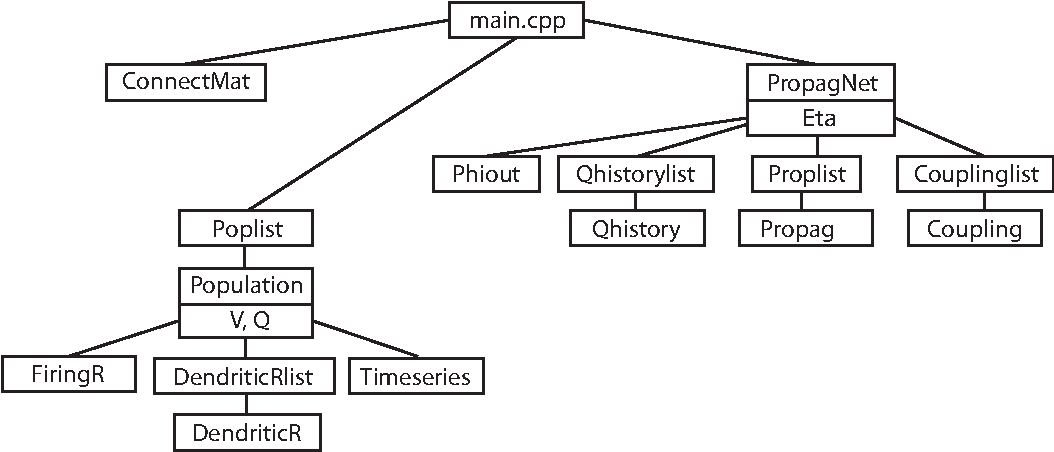
\includegraphics[scale=.8]{class.pdf}\caption{Schematic of the main class structure of \type{NeuroField}. Here, \type{V}, \type{Q}, and \type{Eta} are 2D arrays of doubles, representing the fields $V_a$, $Q_a$, and $\phi_{ab}$.}\label{fig:class}\end{center}\end{figure}

\subsection{Main integration loop}

The main integration loop is coded in \type{main.cpp}. It is schematically illustrated as follows.

\begin{figure}[h!]\begin{center}
\begin{tabular}{ | l l p{12cm} | }
\hline \\

\type{main()}& $\Rightarrow$ &\type{PropagNet::stepQtoP(); Poplist::stepPops(); PropagNet::output() }\\[6pt]

\type{stepQtoP()}& $\Rightarrow$ &
\type{ Qhistorylist::updateQhistories() $\Rightarrow$ QHistory::updateQhistory(); }\\
&&\type{ Proplist::step() $\Rightarrow$ Propag::stepwaveeq(); } \\
&&\type{ Couplinglist::updateP() $\Rightarrow$ Couple::updatePa() }\\[6pt]

\multirow{2}{*}{\type{stepPops()}}&\multirow{2}{*}{$\Rightarrow$}&
\type{Timeseries::get()} if population is stimulus \\
&& \type{Population::stepPop()} if normal population \\[6pt]

\type{stepPop()} & $\Rightarrow$ & \type{ DendriticRlist::stepVa(); DendriticRlist::SumAfferent(); FiringR::getQ() } \\[6pt]

\type{output()}&$\Rightarrow$& \type{Phiout::output(); Couplinglist::output() $\Rightarrow$ Couple::output() }\\

\\\hline
\end{tabular}
\caption{Main integration loop. We use the semicolon to denote a succession of functions, and \type{a()} $\Rightarrow$ \type{b()} symbol to denote function \type{b()} as content of function \type{a()}.}\label{fig:main-loop}
\end{center}\end{figure}

\begin{itemize}
\item One integration step of the model implements the following stages: 1) Firing response/\linebreak stimulus response. 2) Wave equation integration step which includes Q delay processing 3) Coupling response 4) Dendritic response 5) Afferent summation.
\item Most of the computational load comes from integrating wave equations and harmonic oscillators within the dendritic responses.
\item Wave equations are integrated by explicit finite differences integration. A nine point spatial stencil is used to reduce high frequency spatial instabilities when driven by random noise. Other parts of code are unaffected by spatial geometry so this can be switched to irregular gridding easily.
\item Harmonic oscillators with dendritic rseponse are integrated using a heavily strength reduced explicit direct integration assuming constant drive. This was more efficient than a constant drive RK4 algorithm which would not be fourth order in any case due to the constant drive. Rennie used a constant drive RK4 for his 1997 code.
\end{itemize}

\subsection{Component manifest}

The source code contains a main code \type{main.cpp} and various components defining classses of the code. Each class contains a header \type{.h} file and main program unit \type{.cpp} file:

\begin{description}
\item[Istrm] A helper class inheriting from an input stream. This class allows some minimal input checking when reading configuration files. The important functions are:
	\begin{enumerate}
	\item validate: check the next text to be read for the intended keyword of input identifier,
	\item optional: check whether an optional parameter keyword is next to be read,
	\item find: search for the i'th instance of a particular keyword,
	\item choose: return a number of corresponding to which character string from a list is being read.
	\end{enumerate}
\item[Random] Generates random numbers for use by time series generating function.
\item[Parameter] A helper calss to store individual parameters and their keyword names.
\item[Connectmat] Reads and store connectivity matrix information which is called by other classes.
\item[Propagnet] A class representing the propagator network, i.e. the simulated brain. This class dispatches update requests to the neural population for dendritic response and firing response, propagation of phi's along synapses and synaptic coupling.
\item[Timeseries] Generated time series for stimulus input and other driven processes such as time modulated coupling strengths.
\item[Proplist] A container object initializing and accessing all propagators in the simulation.
\item[Poplist] A container for initializing and holding all neural population objects in the simulation.
\item[Population] A class containing firing response and dendritic response information for a given neural population.
\item[Firingr] A class containing firign response and dendritic response information for a given neural population.
\item[Dendriticrlist] A container calss of dendritic responses terminating on a particular neural population.
\item[Dendriticr] A class containing dendritic response from a given population to another population.
\item[Propag] An abstract base class providing a uniform interface for all propagators to be accessed when stepping forward the code. All propagator types must inherit from this class.
\item[Pmap] A class to provide the ``Mapping" propagator behaviour.
\item[Pharmonic] A class to provide the ``Harmonic"---harmonic oscillator behaviour propagator. This si typically used for spatially uniform simulations as it is more efficient than a wave equation propagtor where the simulation will have no spatial variation.
\item[Eqnset] A class to provide the ``Eqnset"---multiple wave equations form of the propagator. This feature has not had significant testing. It uses the helper classes Prefact, Field and Weqn.
\item[Prefact] A helper class for Eqnset to calculate some prefactors used in the calculations of Eqnset.
\item[Field] A helper class to hold Phi field information for waveeqn and Eqnset (via Weqn).
\item[Weqn] A helper class for propagators to store infromation about Tau, the axonal delays associated wtih propagators.
\item[Qhistorylist] A container object initializing and accessing Qhistory objects. These store time history of firing rates.
\item[Qhistory] A container object containing time history information for firing rate Q. It is necessary to store time history information of firing rates since propagtors such as the wave equation and mapping operator are time delayed due to propagation time along axons.
\item[Couplinglist] A container object for initializing and holding synaptic coupling objects.
\item[Couple] An abstract base class providing an interface for synaptic coupling objects. All objects which handle synaptic coupling must inherit from this object.
\item[Coupling] A class which provides synaptic coupling with constant synaptic strengths.
\item[Modcouple] A class which provides synaptic coupling following a model proposed by Clearwater-Rennie for modelling neurotransmitter dynamics.
\item[STDP] A coupling class implementing linear STDP plasticity.
\item[CaDP] A coupling class implementing calcium dependent plasticity.
\item[Modsigma] A class to allow the variance dynamics, modulated sigma model of firing response. This class is still in the testing phase.
\item[Modtheta] A class to model a varying theta (firing threshold). This model was proposed by Kim-Wu.
\item[Modtheta1] A class to model a varying theta (firing threshold). This is a later variant of a model proposed by Kim-Wu.
\item[Phiout] A class to output phi information from the simulation.
\end{description}

\subsection{Submission to svn}

\section{Known bugs or flaws}
According to Peter Drysdale:
\begin{itemize}
\item Code only runs for initial time set to zero. This only effects the stimulus routines.
\item Inadequate range of stimulus patterns currently implemented.
\item Documentation needs to be worked on.
\item Code needs more commenting.
\end{itemize}

\section{TODO}
\begin{enumerate}
\item document switches in exe
\item no need to rename neurofield.dump to neurofield.conf in restart mode?
\item implement restart mode in launcher script?
\item no need for NeuroField write defaults option?
\item tidy up helper scripts
\end{enumerate}
\end{document}
